\documentclass[a4paper,troispoints,pdf,colorBG,slideColor]{prosper}
%\hypersetup{pdfpagemode=FullScreen}

\usepackage{pstricks,pst-node,pst-tree}
\usepackage{amssymb,latexsym}
\usepackage{graphicx}
\setlength{\topmargin}{-0.5in}
\setlength{\textwidth}{9in}
\setlength{\oddsidemargin}{0in}
\setlength{\evensidemargin}{0in}

\newcommand{\ns}[1]{\vfill \end{slide}\begin{slide}{#1}}
\newcommand{\bi}{\begin{itemize}}
\newcommand{\ei}{\end{itemize}}
\newcommand{\Show}[1]{\psshadowbox{#1}}
\newcommand{\graphic}[3]{
\begin{pspicture}(0,0)(0,0)
\rput(#1){\resizebox{#2}{!}{\includegraphics{#3}}}
\end{pspicture}
}
\newcommand{\graphicbox}[3]{
\begin{pspicture}(0,0)(0,0)
\rput(#1){\fbox{\resizebox{#2}{!}{\includegraphics{#3}}}}
\end{pspicture}
}

\newpsobject{showgrid}{psgrid}{subgriddiv=1,griddots=10,gridlabels=6pt}

\title{Video Games Blockbusters}
\author{Geoffrey Matthews\\
based on \href{http://en.wikipedia.org/wiki/}{\em Wikipedia} articles}
\institution{Western Washington University}

\begin{document}
\maketitle

\begin{slide}{Blockbusters}

\begin{pspicture}(0,0)(0,0)
\rput(9,-4){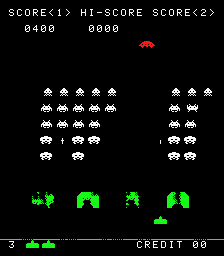
\includegraphics[scale=0.75]{SpaceinvadersArcade.eps}}
\end{pspicture}

{\em Space Invaders}
\bi
\item Introduced to US in 1978
\item First big Japanese success
\item Introduced the ``High Score'' list
\ei

\ns{Blockbusters}

\begin{pspicture}(0,0)(0,0)
\rput(9,-4){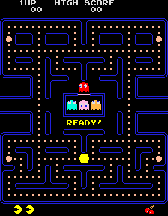
\includegraphics[scale=0.75]{pacman.eps}}
\end{pspicture}
{\em Pac-Man}
\bi
\item American debut 1981
\item Attempt to create non-violent game
\item Generated \$100 million in sales
\ei

\ns{Blockbusters: Tetris}
\begin{pspicture}(0,0)(0,0)
\rput(9.75,-2.5){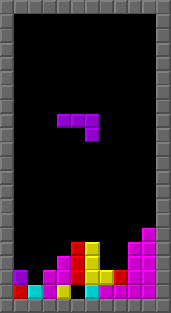
\includegraphics[scale=0.5]{tetris.eps}}
\end{pspicture}
{\scriptsize
\bi
\item Created by Alexy Pajitnov in 1985
\item {\em Andromeda} sold the rights to {\em Spectrum Holobyte}
\item But {\em Andromeda} never settled the deal with Pajitnov
\item {\em Specturm Holobyte} releases the game in 1986
\item {\em Andromeda} continues to sell rights they don't have
\item {\em Nintendo} buys rights from Russia
\item {\em Tengen} (a division of {\em Atari}) develops it for NES
\item {\em Nintendo} claims {\em Atari} stole it;
{\em Atari } sues {\em Nintendo}
\item Courts rule:  {\em Nintendo} wins
\item Game makes {\em Game Boy} phenomenon
\ei
}


\ns{Blockbusters}
\begin{pspicture}(0,0)(0,0)
\rput(8,-4){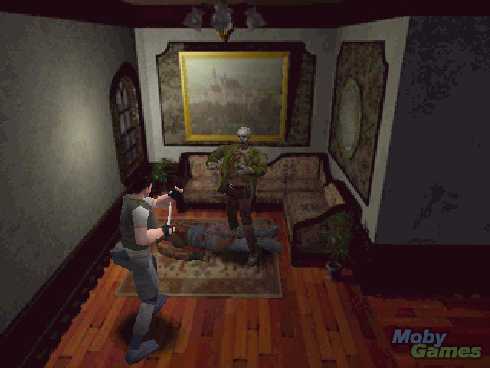
\includegraphics[scale=0.5]{residentevil.eps}}
\end{pspicture}
{\em Resident Evil} by {\em Capcom}
\bi
\item 1996
\item Survival horror
\item Movies 2002, 2004, 2007
\ei

\ns{Blockbusters}
\begin{pspicture}(0,0)(0,0)
\rput(10,-1.5){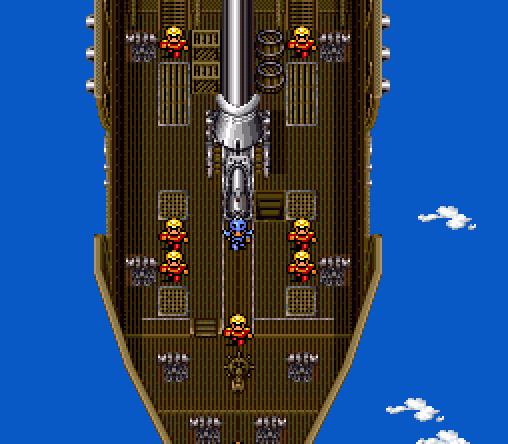
\includegraphics[scale=0.25]{ff4.eps}}
\rput(8,-5){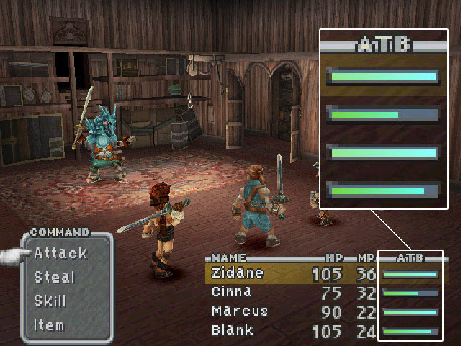
\includegraphics[scale=0.333]{ff9.eps}}
\end{pspicture}
{\em Final Fantasy} by {\em Square Enix}
\bi
\item Released in 1987 to stave off bankruptcy
\item 4th best selling franchise of all time; \\
  (follows {\em Mario}, {\em Pok\'emon}, {\em Sims})
\item 70 million units sold
\item About 28 games in the franchise
\ei

\ns{Blockbusters}
\begin{pspicture}(0,0)(0,0)
\rput(8,-4){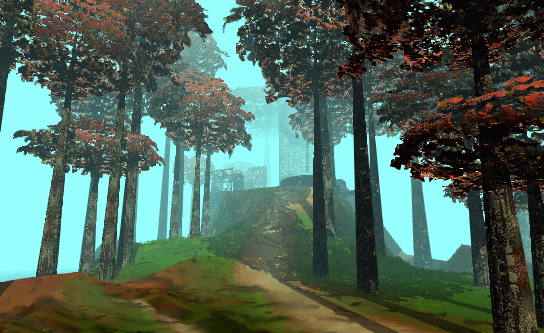
\includegraphics[scale=0.5]{myst.eps}}
\end{pspicture}
{\em Myst} by {\em Cyan}
\bi
\item 1993
\item A game for adults
\item Beginning of the CD-ROM age
\item Most popular computer game (until {\em Sims})
\ei

\ns{Blockbusters}
\begin{pspicture}(0,0)(0,0)
\rput(9.5,-1){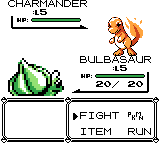
\includegraphics[scale=0.75]{pokemon.eps}}
\end{pspicture}
{\em Pok\'emon}
\bi
\item Created by Satoshi Tajiri
\item Interlinkable {\em Game Boy} game
\item Released 1996
\item 2nd best selling franchise of all time, \\ after {\em Mario}
\item {\em Monster in my Pocket} already trademarked
\item Anime spinoffs
\ei

\ns{Blockbusters: \\Mario}
\begin{pspicture}(0,0)(0,0)
\rput(9,-4){
\includegraphics{mario.eps}}
\end{pspicture}
\bi
\item Biggest franchise of all time
\item 193 million units sold
\item Over 200 games
\item 1991: {\em Donkey Kong}
\item 2007: {\em Super Paper Mario}
\ei

\ns{Blockbusters}
\begin{pspicture}(0,0)(0,0)
\rput(8,-5.25){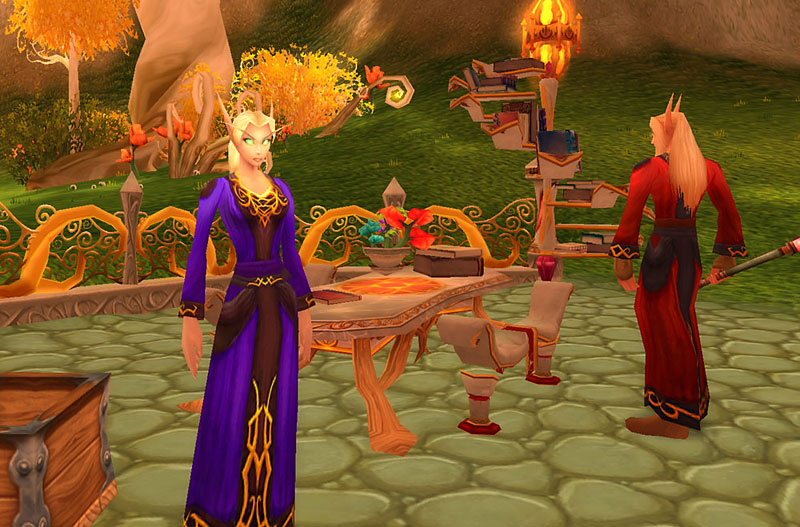
\includegraphics[scale=0.4]{wow.eps}}
\end{pspicture}
{\em World of Warcraft}, 2004
\bi
\item Spinoff from {\em Warcraft: Orcs \& Humans}, 1994
\item MMORPG: 8.5 million online players
\item ``{\em WoW} is the new golf.''
\ei


\ns{\large The Art of Computer Game Design}
{\footnotesize
I dreamed of the day when computer games would be a viable medium of
artistic expression --- an art form. I dreamed of computer games
expressing the full breadth of human experience and emotion. I dreamed
of computer games that were tragedies, games about duty and honor,
self-sacrifice and patriotism. I dreamed of satirical games and
political games; games about the passionate love between a boy and
girl, and the serene and mature love of a husband and wife of decades;
games about a boy becoming a man, and a man realizing that he is no
longer young. I dreamed of games about a man facing truth on a dusty
main street at high noon, and a boy and his dog, and a prostitute with
a heart of gold.
\hfill --- \sl Chris Crawford, 1984
}

\end{slide}
\end{document}
